\documentclass[fontsize=12pt]{scrartcl}
\usepackage[ngerman]{babel}
\usepackage[utf8]{inputenc}
%\usepackage[latin1]{inputenc}
\usepackage{amsmath}
\usepackage{amstext}
\usepackage{amssymb}
\usepackage{stmaryrd}
\usepackage{verbatim}
\usepackage{mathrsfs}
\usepackage{extarrows}
\usepackage[arrow, matrix, curve]{xy}
\usepackage[centering,includeheadfoot,margin=2cm]{geometry}
\usepackage{gensymb}
\usepackage{graphicx}
\usepackage{framed}
\usepackage{xcolor}
\usepackage{float}
\usepackage{graphicx} 
\usepackage{sidecap}
\usepackage{blindtext,wrapfig}
\usepackage{epstopdf}
\usepackage{import}
\usepackage{fancyhdr}
\usepackage{fancybox}
\usepackage{paralist}
\usepackage{graphicx}
\usepackage{caption}
\usepackage{subcaption}
\renewcommand{\l}{\left\vert}
\renewcommand{\r}{\right\vert}
\newcommand{\define}{\ensuremath{\mathrel{\mathop:}=}} % hübscheres :=, da = zentriert wird relativ zu :
\newcommand{\enifed}{\ensuremath{=\mathrel{\mathop:}}} % hübscheres =:, da = zentriert wird relativ zu :
\DeclareGraphicsRule{.tif}{png}{.png}{`convert #1 `basename #1 .tif`.png} 
\pagestyle{fancy}
\fancyhf{}
\fancyhead[R]{Physikalisches Praktikum 1}
\fancyhead[L]{Gentian Rrafshi}
\fancyfoot[R]{\thepage}
\fancyfoot[L]{\today}
\parindent 0pt
\parskip 12pt
\begin{document}

\begin{minipage}{0.9\textwidth}
\begin{center}\large
\title{ S20 Kugelfallviskosimeter \\
		~\\
		~\\
		Assistent: \\ Teresa Schaller \\
		~\\
		Datum Versuchsdurchführung: \\
		07.07.2015}

\author{bearbeitet von\\
		Gruppe 3-031: \\
		Gentian Rrafshi Matrnr. 2721617 }
\date{\today}

\maketitle

\end{center}
\end{minipage}

\newpage

\tableofcontents

\newpage
\noindent

\section{ Versuchsziel}

Ziel des Versuchs ist die Bestimmung der Viskosität eines Pumpenöls in Abhängigkeit zur Temperatur.

\section{ Grundlagen}

Eine wichtige Konstante in diesem Versuch ist die sogenannte Reynolds-Zahl. Diese ist definiert durch 
\begin{equation*}
R=\frac{\rho\cdot v\cdot d}{\eta} = \frac{v\cdot d}{\nu}
\end{equation*}
Wobei hier $\rho$ die Dichte der Flüssigkeit, $v$ die Strömungsgeschwindigkeit der Flüssigkeit, welche einem Körper der charakteristischen Länge $d$ entgegenströmt und $\eta$ bzw. $\nu$ sind jeweils die dynamische bzw. kinema	tische Viskosität. \par

Die Reynolds-Zahl wird oft in der Strömungslehre gebraucht. So beschreibt die \\ Ähnlichkeitsgesetze, wie man Modelle von hydraulisch großer 
Strömungsmaschinen bauen kann, die dennoch das selbe Strömungsverhalten aufweisen. Eines dieser Ähnlichkeiten ist das sogenannte dynamische 
Ähnlichkeit. Diese besagt, dass Modelle sich stömungstechnisch wie die Originale verhalten, wenn die Reynoldszahl identisch gewählt werden kann.\par

Bei der Definition der Reynoldszahl für Flüssigkeiten sieht man den Zusammenhang zwischen dynamischer und kinematischer Viskosität. Dieser zeigt, dass die beiden sich nur von der Dichte der Flüssigkeit abhängen und zwar sogar linear.
\begin{equation*}
\eta = \nu \cdot \rho
\end{equation*}
Da die Dichte temperaturabhängig ist, wird hier auch eine Zusammenhang zwischen dynamischer Viskosität und Temperatur ersichtlich. Anders als bei Gasen nimmt aber die Viskosität mit steigender Temperatur ab. Hierbei gilt dann für die Viskosität:
\begin{equation*}
\eta(T)=\eta_{\infty}\cdot e^{\frac{\Delta E}{k_B \cdot T}}
\end{equation*}
Hier ist $\frac{\Delta E}{k_B}$ die Aktivierungsenergie und $k_B$ die Boltzmann-Konstante. Für den Grenzfall 
\begin{equation*}
\lim\limits_{T \rightarrow \infty} \eta(T)	 = \eta_{\infty}
\end{equation*}
erhält man dann die kleinstmögliche Viskosität $\eta_{\infty}$.\par

Für diesen Versuch gibt es eine empirische Formel für die Viskosität. Diese lautet:
\begin{equation*}
\eta(\bar{T})=K(\rho_K-\rho_{fl})\cdot\bar{T}
\end{equation*}
Im Verlauf des Protokolls wird untersucht, ob diese empirischen mit der theoretischen Formel übereinstimmt. Wobei hier $\bar{T}$ die mittlere Fallzeit der Kugel im Fallrohr ist.
\newpage

\section{Versuchsaufbau und Durchführung}

\subsection{benötigte Geräte}
\begin{figure}[H]
\centering
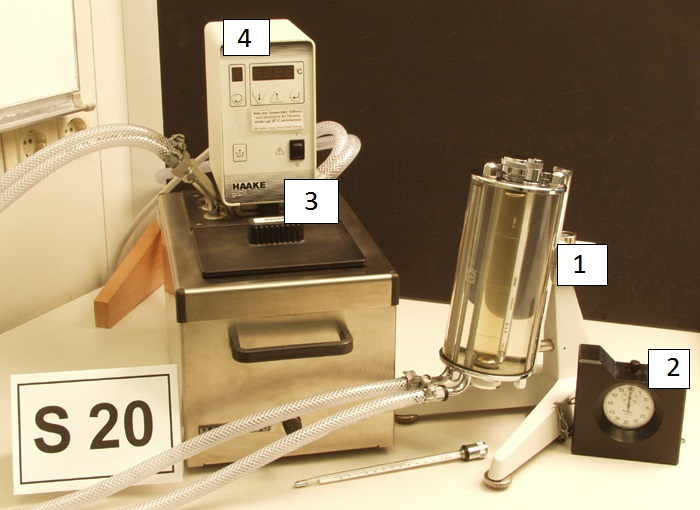
\includegraphics[width=0.7\textwidth]{Graphik/Versuch}
\caption{Versuchsaufbau}
\end{figure}
\begin{itemize}
\item[•] Kugelfall-Viskosimeter (Kästchen 1)
\item[•] Stoppuhr (Kästchen 2)
\item[•] Pumpenöl-Wasser-Bad (Kästchen 3)
\item[•] Thermostat (Kästchen 4)
\end{itemize}

\subsection{Versuchsdurchführung}

Das Fallrohr (Kästchen 1) enthält in innerem eine Kugel. Durch wenden um 180$^{\circ}$ fällt diese Kugel und die Fallzeit wird mit der Stoppuhr (Kästchen 2) gemessen. Dieser Vorgang wird für 5 verschieden Temperaturen jeweils 5 mal durchgeführt. Das Thermostat (Kästchen 4), welches am Pumpenöl-Wasser-Bad (Kästchen 3) angebracht ist, wird hierbei zur Temperaturmessung genommen.
\newpage

\section{Formeln}

\subsection{Formel für die mittlere Zeit}
\begin{equation}
\bar{T}= \frac{\sum_{k=1}^n t_k}{n}
\label{t}
\end{equation}
Wobei $t_k$ [s] die jeweilige Zeitmessung $n$ Messungen und $\bar{T}$ [s] die daraus resultierende mittlere Zeit.

\subsection{empirische Formel für die Viskosität }
\begin{equation}
\eta(\bar{T})=K(\rho_K-\rho_{fl})\cdot\bar{T}
\label{emp}
\end{equation}
Hier ist $K=0,5445\,\frac{\text{mPa}\cdot\text{cm}^3}{\text{g}}$; $\rho_K =8,141\,\frac{g}{\text{cm}^3}$ die Dichte der Kugel und $\rho_{fl} =0,86\,\frac{g}{\text{cm}^3}$ die Dichte des Pumpenöls. $\eta(t)$\,[mPa$\cdot$s] ist dann die Viskosität und $\bar{T}$\,[s] die Fallzeit der Kugel.

\subsection{Formel für die Viskosität }
\begin{equation}
\eta(T)=c_1 e^{\frac{c_2}{T}}
\label{vis}
\end{equation}
Mit $c_1$\,[mPa$\cdot$s],$c_2$\,[K] Materialkonstanten und $T$\,[K] als Temperatur des Pumpenöls. Auch hier ist $\eta(T)$\,[mPa$\cdot$s] die Viskosität.
\newpage

\section{ Messwerte}
\begin{figure}[H]
\centering
\caption{Messwerte}
\begin{tabular}{|c|c|c|c|c|c|} \hline
Temperatur & \multicolumn{5}{c|}{verschiedene Zeitmessungen} \\ \hline
T [$^{\circ}$C]	& $t_1$ [s] & $t_2$ [s]	& $t_3$ [s]	 & $t_4$ [s]	& $t_5$ [s] \\ \hline
35,30	&24,09	&24,02	&23,98	&24,02	&24,00 \\ \hline
40,00	&19,00	&19,93	&19,09	&18,99	&19,04 \\ \hline
45,40	&14,40	&14,57	&14,39	&14,44	&14,46 \\ \hline
50,00	&12,05	&11,93		&11,94		&12,03	&11,97 \\ \hline
55,00	&9,37		&9,44		&9,36		&9,48		&9,40 \\ \hline
60,00	&7,91		&8,05		&8,08		&8,03		&8,03 \\ \hline
\end{tabular}				
\end{figure}
\newpage

\section{ Auswertung}

\subsection{Berechnung mittlere Fallzeit}

Im ersten Teil der Auswertung wird die mittlere Fallzeit der Kugel mit Formel (\ref{t}) berechnet. Beispielhaft wird dies hier mit der Messung für $T=60\,^{\circ}$C ausgeführt. Man erhält:
\begin{align*}
\bar{T}= \frac{\sum_{k=1}^5 t_k}{5} =  \frac{(7,91+8,05	+8,08	+8,03+	8,03)\,\text{s}}{5}=8,02\,\text{s}
\end{align*}
Die anderen errechneten Fallzeiten werden hier tabellarisch aufgeführt:
\begin{figure}[H]
 \vspace{-12pt}
\centering
\caption{Ergebnisse für mittlerer Fallzeit}
\begin{tabular}{|c|c|c|c|c|c|} \hline
\rule{0pt}{12pt} Temperatur T [$^{\circ}$C]	&mittlere Fallzeit $ \bar{T}$ [s] \\ \hline
35,30	&24,02\\ \hline
40,00	&19,21\\ \hline
45,40	&14,45\\ \hline
50,00	&11,98\\ \hline
55,00	&9,41\\ \hline
60,00	&8,02\\ \hline
\end{tabular}				
\end{figure}

\subsection{Berechnung der Viskosität nach empirischer Formel}

Mit Hilfe von Formel (\ref{emp}) und dem mittleren Fallzeit $\bar{T}$ kann man nun die Viskosität errechnen. Auch hier wird dies an einer Beispielrechnung nochmal verdeutlicht. Wieder für $T=60\,^{\circ}$:
\begin{align*}
\eta(\bar{T})=K(\rho_K-\rho_{fl})\cdot\bar{T}=0,5445\,\frac{\text{mPa}\cdot\text{cm}^3}{\text{g}}(8,141\,\frac{g}{\text{cm}^3}- 0,86\,\frac{g}{\text{cm}^3})\cdot8,02\,\text{s}=31,80\,\text{mPa}\cdot\text{s}
\end{align*}
Die restlichen Werte sind in der nachfolgenden Tabelle nachlesbar:
\begin{figure}[H]
 \vspace{-12pt}
\centering
\caption{Ergebnisse für Viskosität}
\label{tab}
\begin{tabular}{|c|c|} \hline
\rule{0pt}{12pt} mittlere Fallzeit $ \bar{T}$ [s] &Viskosität $\eta(\bar{T})$ [s] \\ \hline
24,02	&95,24 \\ \hline
19,21	&76,16 \\ \hline
14,45	&57,30 \\ \hline
11,98	&47,51 \\ \hline
9,41		&37,31 \\ \hline
8,02		&31,80 \\ \hline
\end{tabular}				
\end{figure}
\newpage

\subsection{Nachweis der Viskositätsgleichung (\ref{vis})}

Zum Nachweis der Gleichung (\ref{vis}) benötigen wir zum einen die errechneten Viskositäten aus Abb.(\ref{tab}) als auch das Inverse der Temperatur in Kelvin. Wir erhalten folgende Tabelle
 \begin{figure}[H]
 \vspace{-12pt}
\centering
\caption{Ergebnisse für Viskosität und Inverse der Temperatur}
\begin{tabular}{|c|c|} \hline
\rule{0pt}{12pt} Inverse der Temperatur $ \frac{1}{T} [\frac{10^3}{\text{K}}] $&Viskosität $\eta(T)$ [s] \\ \hline
3,24	&95,24 \\ \hline
3,19	&76,16 \\ \hline
3,14	&57,30 \\ \hline
3,09	&47,51 \\ \hline
3,05	&37,31 \\ \hline
3,00	&31,80 \\ \hline
\end{tabular}				
\end{figure}
Dadurch ergibt sich folgendes $\frac{1}{T}-\eta(T)$-Diagramm, wobei die $\eta(T)$-Achse logarithmiert dargestellt wird:
\begin{figure}[H]
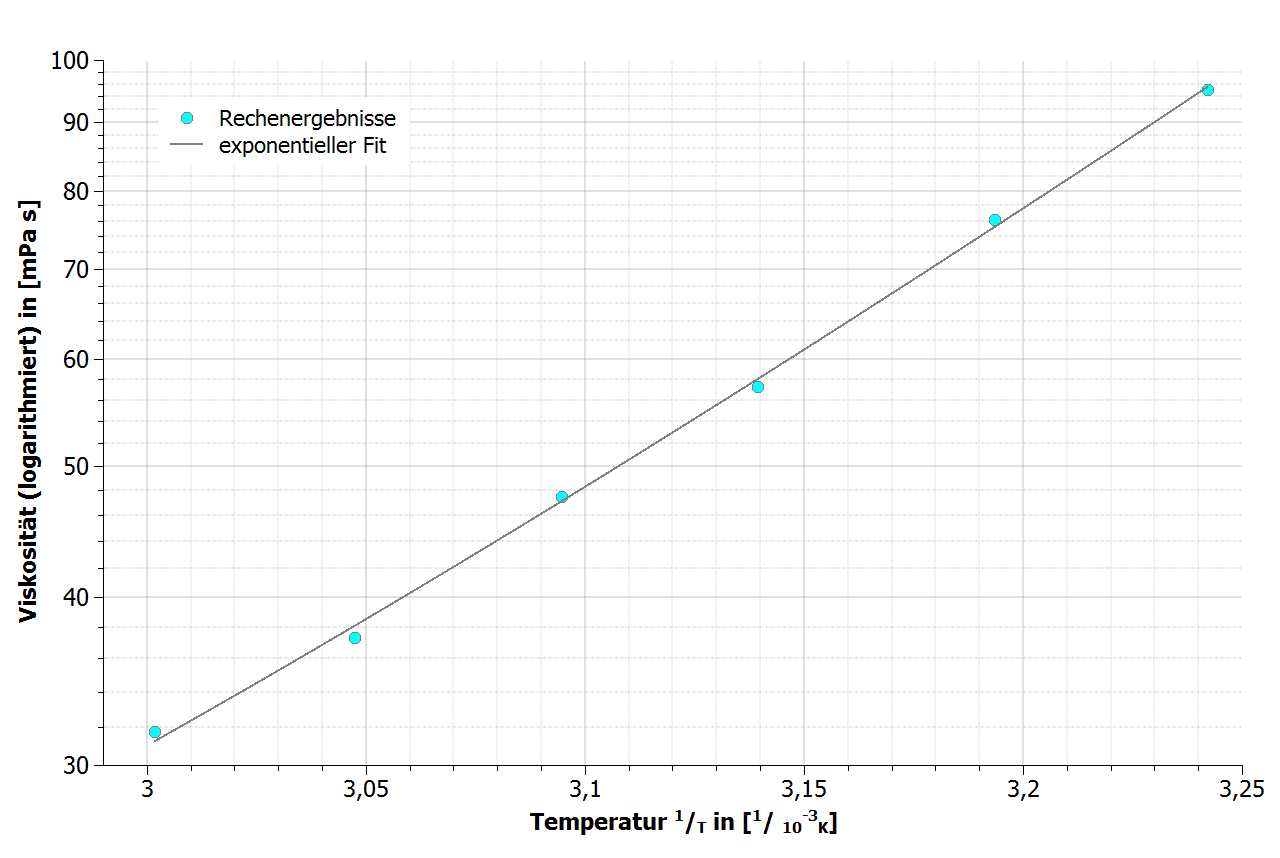
\includegraphics[width=1\textwidth]{Graphik/Eta}
\end{figure}

\newpage

Durch einen exponentiellen Fit $f(x)=a\cdot e^{b\cdot x}$ in QTI-Plot durch die Ergebnisse erhält man dann für die Materialkonstanten:
\begin{itemize}
\item[] a=c$_1$=$2,12\cdot 10^{-05}$\,mPa$\cdot$s
\item[] b=c$_2$=$4725,09$\,K
\end{itemize}
In diesem Fall erhält man also als Gleichung:
\begin{equation*}
\eta(T)=c_1 e^{\frac{c_2}{T}}=\eta(T)=2,12\cdot 10^{-05}\,\text{mPa$\cdot$s} \cdot e^{\frac{4725,09\,\text{K}}{T}}
\end{equation*}
\newpage

\section{Fehlerrechnung}

\subsection{Fehler bei Viskosität}

Der Fehler für die Viskosität kann mit Hilfe von Formel (\ref{emp}) bestimmt werden. Als Fehler kann die menschliche Reaktionszeit von $\Delta T=$0,5\,s  angenommen werden. Dieser hebt sich durch mitteln der Zeit nicht auf. Es gilt dann:
\begin{align*}
\Delta\eta &= \l K(\rho_K-\rho_{fl}) \frac{\partial}{\partial \bar{T}}\bar{T}\r\cdot \Delta T= \l K(\rho_K-\rho_{fl})\r\cdot \Delta T
\end{align*}
Und man erhält als Fehler für $\Delta\eta$:
\begin{align*}
\Delta\eta  = \l0 ,5445\,\frac{\text{mPa}\cdot\text{cm}^3}{\text{g}}(8,141\,\frac{g}{\text{cm}^3}- 0,86\,\frac{g}{\text{cm}^3})\r \cdot 0,5\,\text{s} = 1,98\,\text{mPa$\cdot$s}
\end{align*}

\subsection{Fehler bei Inverse der Temperatur}

Im Prinzip können wir einen Fehler von $\Delta T=1K$ annehmen. Dadurch ergibt sich als Fehler für $\Delta\frac{1}{T}$:
\begin{align*}
\Delta\frac{1}{T}= \l \frac{\partial}{\partial T} \frac{1}{T} \r \cdot \Delta T = \l \frac{-1}{T^2} \r \cdot \Delta T =  \frac{1}{T^2} \cdot \Delta T
\end{align*}
Auch hier wird eine Beispielrechnung aufgeführt für $\frac{1}{T}=3,24\cdot \frac{10^3}{\text{K}}$. Im Anschluss werden dann die restlichen Werte in einer Tabelle dargestellt:
\begin{align*}
\Delta\frac{1}{T}&=  \frac{1}{T^2} \cdot \Delta T
= 3,24^2\cdot \frac{10^6}{\text{K}^2} \cdot 1\,\text{K}
=10,51\,\frac{10^6}{\text{K}}
\end{align*}
 \begin{figure}[H]
 \vspace{-12pt}
\centering
\caption{Ergebnisse für Viskosität und Inverse der Temperatur}
\begin{tabular}{|c|c|} \hline
\rule{0pt}{12pt} Inverse der Temperatur $ \frac{1}{T} [\frac{10^3}{\text{K}}] $& Fehler $\Delta\frac{1}{T} [\frac{10^6}{\text{K}}]$ \\ \hline
3,24	&10,51 \\ \hline
3,19	&10,20 \\ \hline
3,14	&9,85 \\ \hline
3,09	&9,58 \\ \hline
3,05	&9,29 \\ \hline
3,00	&9,01 \\ \hline
\end{tabular}				
\end{figure}
Beide, $\Delta\eta$ und $\Delta\frac{1}{T}$, werden als Fehlerbalken in ein Diagramm am Ende der Fehlerrechnung hinzugefügt.

\subsection{Fehler in den Materialkonstanten}

Mit Hilfe von QTI-Plot erhält man $f_{\text{min}}$ und $f_{\text{max}}$. In diesem Fall erhält man:
\begin{align*}
\eta_{\text{max}}(T) &=0,24\cdot 10^{-05}\,\text{mPa$\cdot$s} \cdot e^{\frac{5439,11\,\text{K}}{T}} \\
\eta_{\text{min}}(T) &=15,12\cdot 10^{-05}\,\text{mPa$\cdot$s} \cdot e^{\frac{4103,36\,\text{K}}{T}}
\end{align*}
Damit erhält man:
 \begin{figure}[H]
 \vspace{-12pt}
\centering
\caption{Fehler für Materialkonstante}
\begin{tabular}{c|c|c} \hline
& Materialkonstante $c_1$ [$10^{-05}$\,\text{mPa$\cdot$s}]& Materialkonstante $c_2$ [\text{K}]\\ \hline
minimaler Fehler &1,88	 &621,73 \\ \hline
maximaler Fehler &13	&714,02 \\ \hline
\end{tabular}				
\end{figure}
und erhalten damit folgendes Diagramm:
\begin{figure}[H]
\vspace{-12pt}
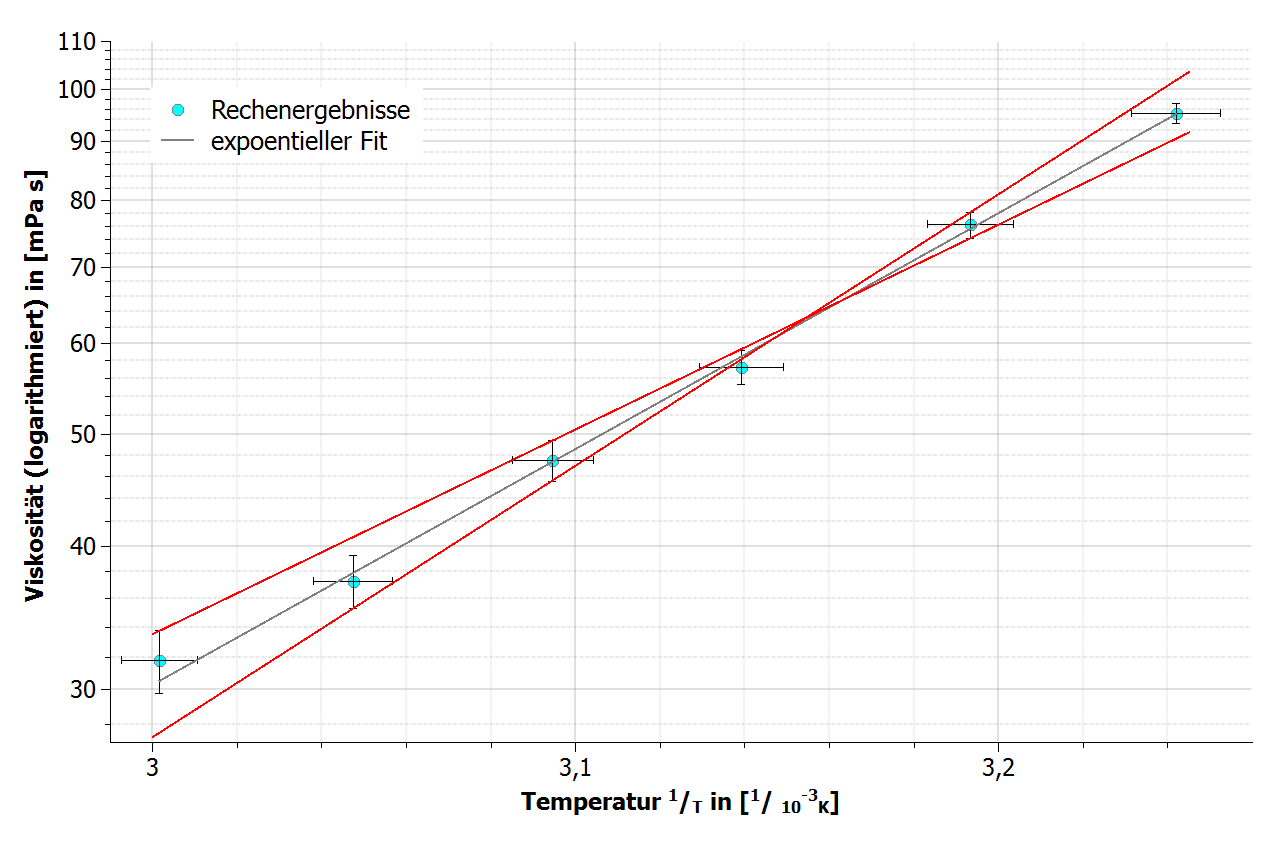
\includegraphics[width=1\textwidth]{Graphik/Etafehler}
\end{figure}

\newpage

\section{Zusammenfassung}

Im ersten Teil des Versuchs sollten wir die Viskosität des Pumpenöls berechnen. Die errechneten Werte sind in folgender Tabelle dargestellt:
 \begin{figure}[H]
 \vspace{-12pt}
\centering
\caption{Zusammenfassung Viskosität und Inverse der Temperatur}
\begin{tabular}{|c|c|c|c|} \hline
\rule{0pt}{12pt} Inverse Temperatur $ \frac{1}{T} [\frac{10^3}{\text{K}}] $& Fehler $\Delta\frac{1}{T} [\frac{10^6}{\text{K}}]$ &Viskosität $\eta(T)$ [\text{mPa$\cdot$s}] & Fehler $\Delta\eta$ [\text{mPa$\cdot$s}] \\ \hline
3,24	&10,51	&95,24	&1,98\\ \hline
3,19	&10,20	&76,16	&1,98\\ \hline
3,14	&9,85		&57,30	&1,98\\ \hline
3,09	&9,58		&47,51	&1,98\\ \hline
3,05	&9,29		&37,31	&1,98\\ \hline
3,00	&9,01		&31,80	&1,98\\ \hline
\end{tabular}				
\end{figure}
Im zweiten Teil des Versuchs soll der exponentielle Zusammenhang zwischen der Viskosität und dem Inversen der Temperatur nachgewiesen werden. Dieser wurde in diesem Versuch auch ersichtlich. In diesem Fall erhält man:
\begin{equation*}
\eta(T)=c_1 e^{\frac{c_2}{T}}=\eta(T)=2,12\cdot 10^{-05}\,\text{mPa$\cdot$s} \cdot e^{\frac{4725,09\,\text{K}}{T}}
\end{equation*}
Für die Fehler in den Materialkonstanten erhält man:
 \begin{figure}[H]
 \vspace{-12pt}
\centering
\caption{Fehler für Materialkonstante}
\begin{tabular}{c|c|c} \hline
& Materialkonstante $c_1$ [$10^{-05}$\,\text{mPa$\cdot$s}]& Materialkonstante $c_2$ [\text{K}]\\ \hline
minimaler Fehler &1,88	 &621,73 \\ \hline
maximaler Fehler &13	&714,02 \\ \hline
\end{tabular}				
\end{figure}
und damit folgende Fehlerkurven:
\begin{align*}
\eta_{\text{max}}(T) &=0,24\cdot 10^{-05}\,\text{mPa$\cdot$s} \cdot e^{\frac{5439,11\,\text{K}}{T}} \\
\eta_{\text{min}}(T) &=15,12\cdot 10^{-05}\,\text{mPa$\cdot$s} \cdot e^{\frac{4103,36\,\text{K}}{T}}
\end{align*}
\newpage
\section{Literaturverzeichnis}

\renewcommand{\refname}{~}
\vspace{-30pt}
\begin{thebibliography}{xx}
   \bibitem[A]{A}  	Graphik aus \textit{\glqq S20 Kugelfallviskosimeter\grqq , in 	\\
   								http://www3.physik.uni-stuttgart.de/studium/praktika/ap/}, \\
   								unter \textit{http://www3.physik.uni-stuttgart.de/studium/praktika/ap/pdf\_dateien/S20.pdf}; \\
   								abgerufen am  13.07.2015
\end{thebibliography}

\section{Anhang}

\end{document}